
\documentclass{beamer}
\usepackage[T1]{fontenc}
\usepackage[utf8]{inputenc}
\usetheme{Boadilla}
\usepackage{amsfonts,amssymb,amsmath,amsthm}
\usepackage{hyperref}
\usepackage{tikz}
\usepackage{bussproofs}
\usepackage{bm} % For bold symbols
\usepackage{xcolor}
\usetikzlibrary{cd,backgrounds}
\renewcommand\mathfamilydefault{\rmdefault} % Nicer math font
\usepackage{caption}
%% 
%% Math symbol definitions
%% 
\newcommand{\N}{\mathbb{N}}
\newcommand{\M}{\mathcal{M}}
\newcommand{\Z}{\mathbb{Z}}
\newcommand{\Oh}{\mathcal{O}}
\newcommand{\F}{\bm{F}}
\newcommand{\C}{\bm{C}}
\newcommand{\D}{\bm{D}}
\newcommand{\h}{\textrm{Hom}}
\newcommand{\op}{{\textrm{op}}}
\newcommand{\hc}{\h_{\bm C}}
\newcommand{\defeq}{:=}
\newcommand{\code}[1]{\texttt{#1}}


%% 
%% Other settings
%% 
\newcommand{\mrk}[1]{{\textcolor{red}#1}}

\hypersetup{
  colorlinks=true,
  linkcolor=blue
}

% Information to be included in the title page:
\title{Formalizing \textit{Proving properties of programs by structural induction} in Agda}
\author{Johannes Ljung Ekeroth, Lukas Skystedt}
\date{October, 2021}

\begin{document}
\beamertemplatenavigationsymbolsempty % Remove navigation buttons
\section{Introduction}
\frame{\titlepage}
\begin{frame}[fragile]
  \frametitle{Overview}
  Paper by R.M Burstall: \textit{Proving properties of programs by structural induction} (available through the \href{https://web.archive.org/web/20201112001546/https://www.cse.chalmers.se/edu/year/2010/course/DAT140_Types/Burstall.pdf}{Wayback Machine}).
\vspace{1em}

  The paper uses a small, informal, untyped functional language with
  \begin{itemize}
  \item Correctness proofs of two functions
    \begin{itemize}
    \item sorting algorithm
    \item simple compiler
    \end{itemize} 
    \pause
  \item We formalize the proofs in Agda. We do not formalize the language.
    \pause
  \item Code available on GitHub:\\ \small \url{https://github.com/Lukas-Skystedt/Burstall-Structural-Deduction-in-Agda}.
  \end{itemize}
\end{frame}

\begin{frame}
  \frametitle{Data types}
  \begin{itemize}
  \item Trees\\
    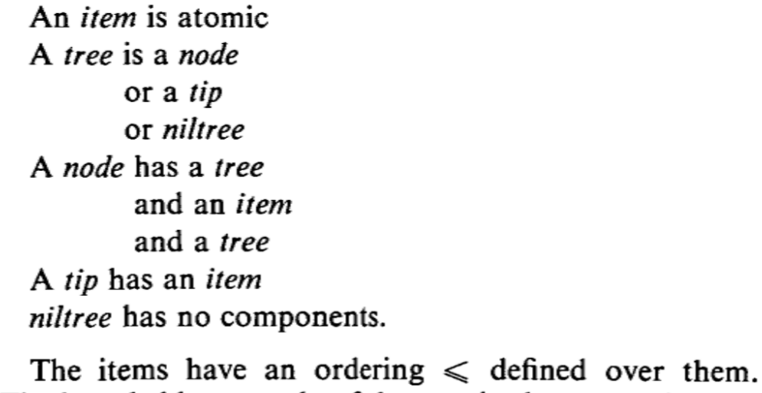
\includegraphics[width=.6\textwidth]{./tree.png}
  \item Lists (\code{::} is sugar for \code{cons})\\
    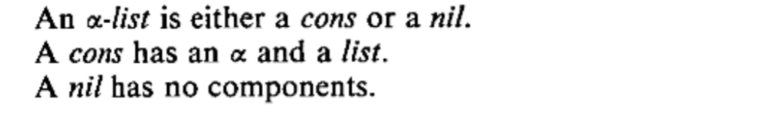
\includegraphics[width=.6\textwidth]{./list.png}
  \end{itemize}
\end{frame} 

\section{Basic definitions and lemmas}
\begin{frame}
  \begin{block}{Basic Functions}
    {\center 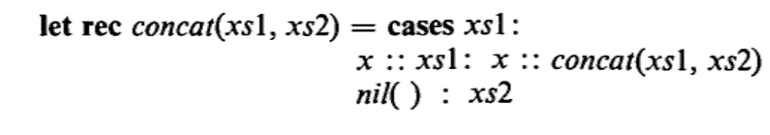
\includegraphics[width=.5\textwidth]{./concat.png}\\
      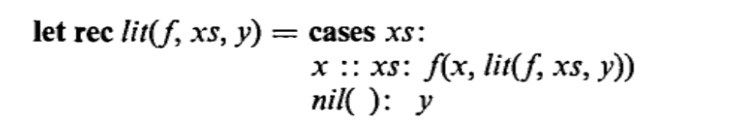
\includegraphics[width=.5\textwidth]{./lit.png}\\}
    Note: \code{lit} is commonly called \code{foldl}.
  \end{block}
  \pause
  \begin{block}{First lemma}
    \center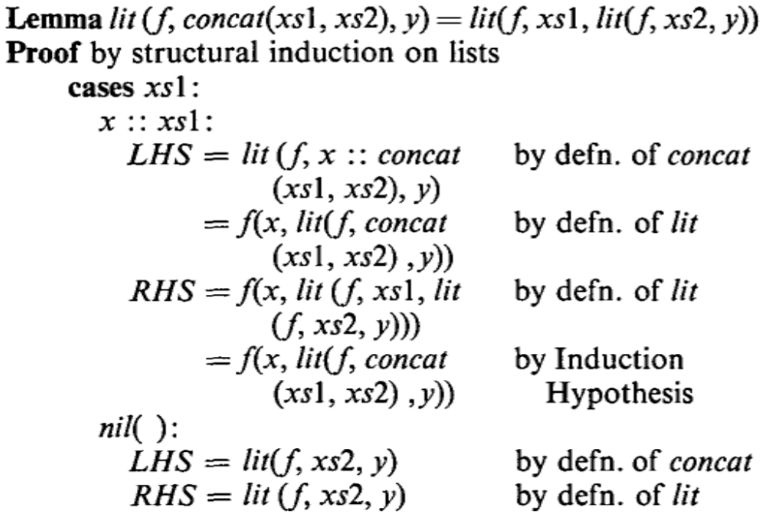
\includegraphics[width=.5\textwidth]{./lit-concat-lemma.png}\\
  \end{block}
\end{frame} 

\begin{frame}
  \frametitle{Trees and Sorting}
  {\center 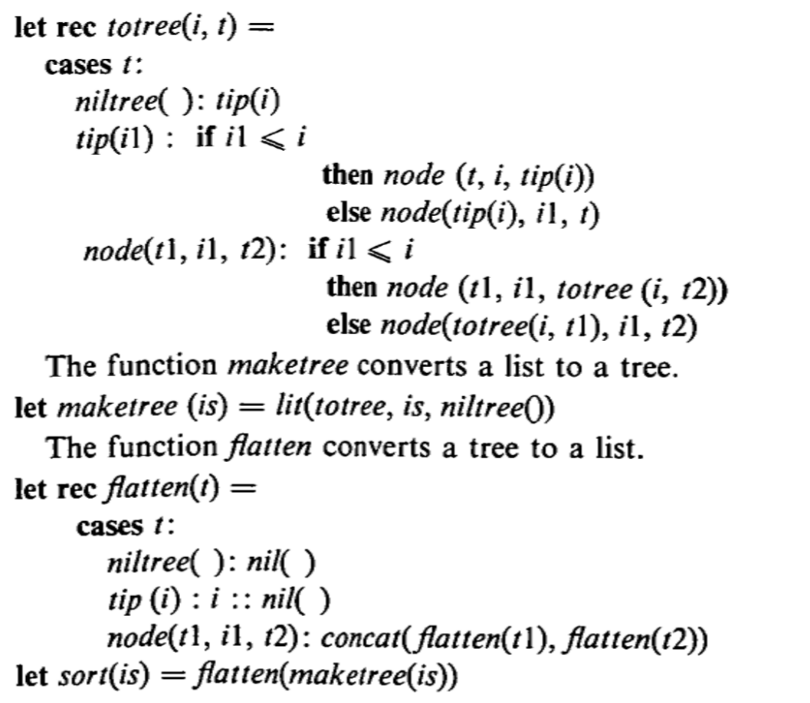
\includegraphics[width=.5\textwidth]{./tree-fns.png}\\}
\end{frame} 

\begin{frame}[fragile]
  \frametitle{Trees}

  \begin{figure}
    \vspace{-2em}
    \caption*{\code{maketree([1,5,2,4,3])}}
    
    \begin{tikzcd}[column sep = 0em]
      nil
    \end{tikzcd}
    \pause
    $\overset{3}{\implies}$
    \begin{tikzcd}[column sep = 0em]
      \mrk 3
    \end{tikzcd}
    \pause
    $\overset{4}{\implies}$
    \begin{tikzcd}[column sep = 0em]
      & \mrk 4\ar[ld, red]\ar[rd,red]\\
      3 && \mrk 4 \\
    \end{tikzcd}
    \pause
    $\overset{2}{\implies}$
    \begin{tikzcd}[column sep = 0em]
      &&& 4\ar[ld, red]\ar[rrd]\\
      && \mrk 3\ar[ld, red]\ar[rd, red] &&& 4 \\
      & \mrk 2 && 3
    \end{tikzcd}
    \pause
    $\overset{5}{\implies}$
    \begin{tikzcd}[column sep = 0em]
      &&&& 4\ar[lld]\ar[rrd, red]\\
      && 3\ar[ld]\ar[rd] &&&& \mrk 5\ar[ld, red]\ar[rd, red] \\
      & 2 && 3 && 4 && \mrk 5
    \end{tikzcd}
    \pause
    $\overset{1}{\implies}$
    \begin{tikzcd}[column sep = 0em]
      &&&& 4\ar[lld]\ar[rrd]\\
      && 3\ar[ld,red]\ar[rd] &&&& 5\ar[ld]\ar[rd] \\
      & \mrk 2\ar[ld,red]\ar[rd,red] && 3 && 4 && 5 \\
      \mrk 1 && 2
    \end{tikzcd}
  \end{figure}
\end{frame}

\section{Correctness of Sorting}
\begin{frame}
  Goal:
  {\center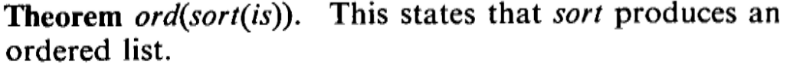
\includegraphics[width=.5\textwidth]{./sort-theorem.png}\\}
  But first, some definitions:\\

  {\center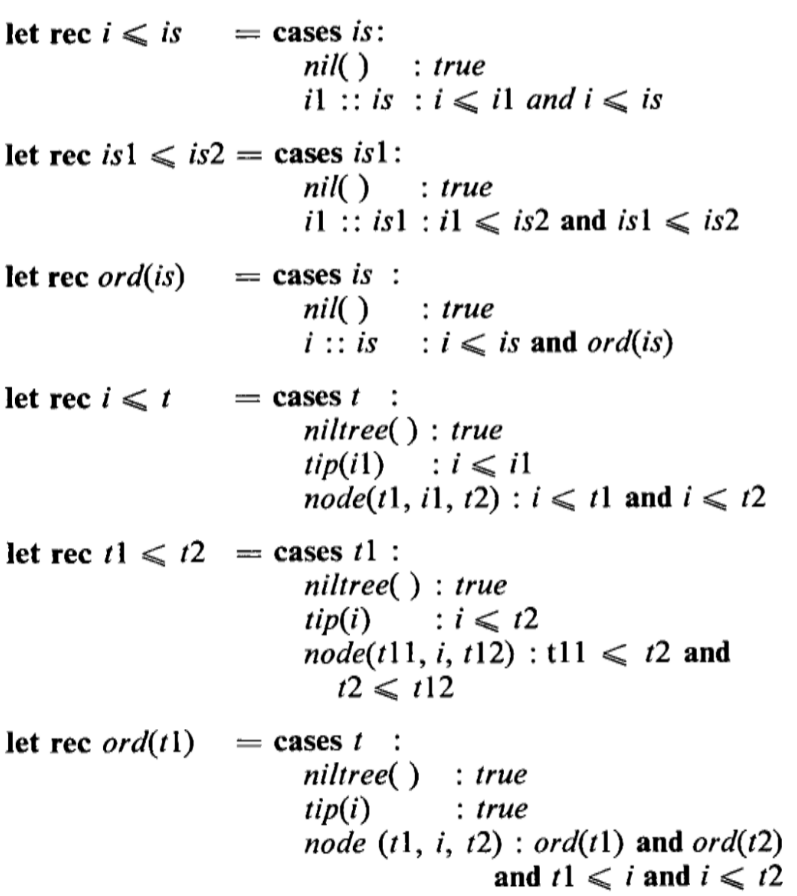
\includegraphics[width=.5\textwidth]{./orderings.png}\\}
\end{frame}
\begin{frame}
  \begin{itemize}
  \item \code{totree} respects ordering\\
    {\center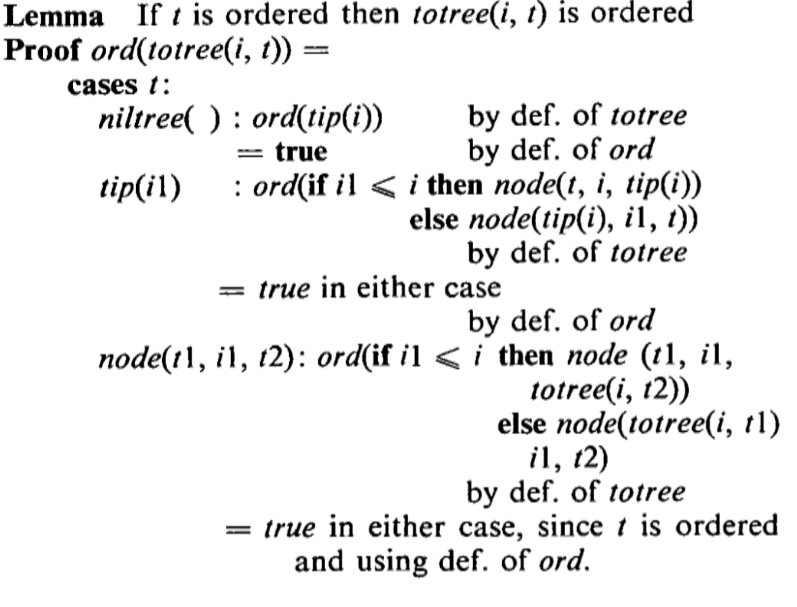
\includegraphics[width=.5\textwidth]{./ord-totree.png}\\}
  \item \code{maketree} respects ordering\\
    {\center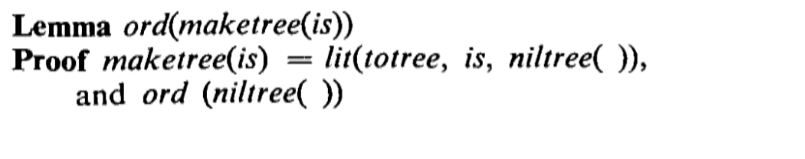
\includegraphics[width=.5\textwidth]{./ord-maketree.png}\\}
  \end{itemize}
\end{frame}
\begin{frame}
  \begin{itemize}
  \item \code{concat}, \code{flatten} also respect ordering.
  \end{itemize}
  {\center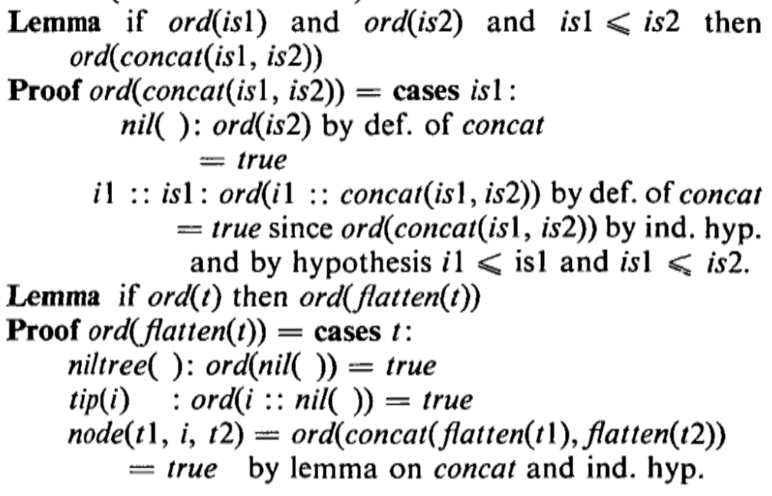
\includegraphics[width=.5\textwidth]{./ord-concat.png}\\}
\end{frame}

\begin{frame}
  \frametitle{Summary}
 % TODO rephrase 
  \begin{itemize}
  \item Formalization can reveal that things that appear trivial, and are
    therefore omitted, are not actually always trivial.
  \item Formalization can help find errors.
  \item Equational reasoning is neat.
  \end{itemize}
\end{frame}
\end{document}

